\documentclass[11pt]{beamer}

\usepackage{fontawesome5}
\usepackage[utf8]{inputenc}
\usepackage[magyar]{babel}
\usepackage[T1]{fontenc}
\usepackage{amsmath, amsfonts, amssymb, graphicx, lmodern, xcolor, hyperref}
\usepackage{animate}

\usepackage[sfdefault]{FiraSans}
\usepackage{FiraMono}
\usepackage{tikz}

\usetheme{CambridgeUS}
\useinnertheme{rounded}
\usefonttheme{professionalfonts}

\definecolor{primary}{RGB}{128, 0, 0} % CambridgeUS maroon
\definecolor{secondary}{RGB}{13, 110, 253} % Bootstrap Primary
\definecolor{accent}{RGB}{255, 193, 7} % Bootstrap Warning
\definecolor{background}{RGB}{248, 249, 250} % Bootstrap Light
\definecolor{text}{RGB}{33, 37, 41} % Bootstrap Dark

\setbeamercolor{normal text}{fg=text, bg=background}
\setbeamercolor{title}{fg=primary}
\setbeamercolor{frametitle}{fg=primary, bg=background}
\setbeamercolor{structure}{fg=secondary}
\setbeamercolor{block title}{fg=white, bg=primary}
\setbeamercolor{block body}{fg=text, bg=background}
\setbeamercolor{item}{fg=secondary}
\setbeamercolor{caption}{fg=accent}
\setbeamercolor{page number in head/foot}{fg=text}


\title{Nyelvi modellek a projektmenedzsmentben}
\subtitle{Mesterséges intelligencia a web- és mobilalkalmazásokban}
\author{Tóth Dorina Ildikó (FYA26Y) \\ Programtervező informatikus BSc \\ Nappali}
\institute{Eszterházy Károly Katolikus Egyetem \\ Matematikai és Informatikai Intézet}
\date{2025}

\logo{
\includegraphics[height=1cm]{ekke_logo.png}}

\setbeamertemplate{footline}{%
    \leavevmode%
    \hbox{%
    \begin{beamercolorbox}[wd=.35\paperwidth,ht=2.25ex,dp=1ex,center]{author in head/foot}%
        \usebeamerfont{author in head/foot}Tóth Dorina Ildikó (FYA26Y)
    \end{beamercolorbox}%
    \begin{beamercolorbox}[wd=.45\paperwidth,ht=2.25ex,dp=1ex,center]{title in head/foot}%
          \usebeamerfont{title in head/foot}\insertshorttitle
    \end{beamercolorbox}%
    \begin{beamercolorbox}[wd=.10\paperwidth,ht=2.25ex,dp=1ex,center]{date in head/foot}%
      \usebeamerfont{date in head/foot}\insertshortdate
    \end{beamercolorbox}}%
    \begin{beamercolorbox}[wd=.10\paperwidth,ht=2.25ex,dp=1ex,center]{date in head/foot}%
        \usebeamerfont{date in head/foot}\insertframenumber{} / \inserttotalframenumber
    \end{beamercolorbox}%
    \vskip0pt%
}
% \setbeamertemplate{footline}{%
%   \hfill%
%   \usebeamercolor[fg]{page number in head/foot}%
%   \usebeamerfont{page number in head/foot}%
%   \insertframenumber\,/\,\inserttotalframenumber%
%   \kern1em\vskip2pt%
% }
% \setbeamercolor{page number in head/foot}{fg=text}

\begin{document}

\begin{frame}
    \setbeamertemplate{footline}{}
    \setbeamertemplate{logo}{}
    \begin{tikzpicture}[remember picture,overlay]
        \node[anchor=center, inner sep=0pt] at (current page.center)
          {
\includegraphics[width=\paperwidth, height=\paperheight, keepaspectratio]{ekke_logo.png}};
        \fill[fill=background, fill opacity=0.9] (current page.south west) rectangle (current page.north east);
    \end{tikzpicture}
    \maketitle
    \begin{center}
        \footnotesize{Témavezető: \begin{tabular}{l} Dr. Kovásznai Gergely \\ Tanszékvezető, egyetemi docens \end{tabular}}
    \end{center}
\end{frame}

\begin{frame}{Tartalomjegyzék}
    \tableofcontents
\end{frame}

\section{Téma rövid bemutatása}
\begin{frame}{Téma rövid bemutatása}
    \begin{itemize}
        \item \textbf{Miről szól a szakdolgozat?}
        \begin{itemize}
            \vspace{0.5em}
            \item Mesterséges intelligencia (MI) szerepe a webalkalmazásokban
            % A szakdolgozatom célja, hogy bemutassam és megismerjem a mesterséges intelligencia szerepét és integrálhatóságát a webalkalmazásokban, különösen az adminisztratív feladatok megkönnyítésében, mint a dokumentációk és specifikációk gyors létrehozása.
        \end{itemize}
        
        \vspace{0.75em}
        
        \item \textbf{Inspirációk}
        \begin{itemize}
            \vspace{0.5em}
            \item Technológiai fejlődés és gyakorlati tapasztalat
            \vspace{0.5em}
            \item MI alkalmazások és lehetőségek
            \vspace{0.5em}
            \item Személyes inspiráció (egyetemi projektmunkák)
            % A témaválasztást a mesterséges intelligencia gyors fejlődése és az ehhez kapcsolódó technológiai kérdések motiválták. Személyes inspirációt jelentett az egyik egyetemi kurzuson végzett projektmunka, amely során a mesterséges intelligencia implementálása során szerzett gyakorlati tapasztalatok formálták az érdeklődésemet.
        \end{itemize}
        
        \vspace{0.75em}
        
        \item \textbf{Célkitűzések}
        \begin{itemize}
            \vspace{0.5em}
            \item Hatékony MI-alapú dokumentumkezelés  
            % A célom egy olyan webalkalmazás létrehozása volt, amely gyorsítja az adminisztratív feladatok elvégzését, különösen a dokumentációk és specifikációk elkészítését nyelvi modellek segítségével.  
            \vspace{0.5em}
            \item Minimális hardverigény  
            % Az ingyenesen elérhető nyelvi modellek hatékony felhasználása alacsony hardverigény mellett. Különböző promptolási technikák tesztelése és optimalizálása.  
            \vspace{0.5em}
            \item Intuitív felhasználói felület  
            % Könnyen kezelhető, áttekinthető interfész, amely támogatja a gyors és hatékony munkavégzést.  
            \vspace{0.5em}
            \item Rugalmas konfiguráció  
            % Különböző nyelvi modellek támogatása, amely lehetővé teszi a felhasználók számára a saját igényeiknek megfelelő beállítások használatát.
        \end{itemize}
    \end{itemize}
\end{frame}

\section{Felhasznált technológiák}
\begin{frame}{Felhasznált technológiák}
    \vspace{-1em}
    \begin{columns}[T]
    \column{0.45\textwidth}
      \begin{block}{\faCode~Implementálás}
        \small
        \begin{itemize}
          \item Django, Python
          \item HTML, CSS, JavaScript
          \item Bootstrap
        \end{itemize}
      \end{block}
      \begin{block}{\faDatabase~Adatbázis}
        \small
        \begin{itemize}
          \item SQLite
        \end{itemize}
      \end{block}
    \column{0.45\textwidth}
      \begin{block}{\faTasks~Munkaszervezés}
        \small
        \begin{itemize}
          \item GitHub Projects
          \item GitHub Issues
        \end{itemize}
      \end{block}
      \begin{block}{\faCodeBranch~Verziókövetés}
        \small
        \begin{itemize}
          \item Git, GitHub
          \item GitHub Desktop
        \end{itemize}
      \end{block}
    \end{columns}
    \vspace{0.5em}
    \begin{columns}[T]
    \column{0.25\textwidth}
    \column{0.5\textwidth}
    \begin{block}{\faRobot~Nyelvi modellek}
        \small
        \begin{itemize}
          \item DistilGPT2
          \item GPT-Neo 125
          \item Facebook OPT 125M, 350M
          \item GPT-2 Medium
        \end{itemize}
      \end{block}
    \column{0.25\textwidth}
    \end{columns}
   		% Az implementáció során a Django és Python alapú backend, valamint a HTML, CSS, JavaScript és Bootstrap alapú frontend technológiák biztosítják a teljes funkcionalitást és felhasználói élményt.
   		% Az adatbázis kezeléséhez az SQLite-ot választottam, amely egy könnyen használható, fájl alapú megoldás, így ideális kisebb alkalmazásokhoz.
   		% A munkaszervezéshez és feladatkövetéshez olyan eszközöket használtam, mint a GitHub Projects és Issues, amelyek lehetővé teszik a projektek hatékony menedzselését és dokumentálását.
   		% A verziókövetéshez Git és GitHub alapú megoldásokat használtam, amelyek biztosítják a kódbázis folyamatos verziókezelését és a kollaboráció támogatását.
   		% A nyelvi modellek kiválasztása során olyan nyílt forráskódú modellek kerültek előtérbe, mint a DistilGPT2, GPT-Neo 125M, Facebook OPT 125M és 350M, valamint a közepes méretű GPT-2, amelyek különböző paraméterekkel és teljesítménnyel rendelkeznek, lehetővé téve a kísérletezést különböző szövegfeldolgozási feladatokkal.
   		
\end{frame}

\section{Az elkészült projekt ismertetése}

\begin{frame}{Adatbázis struktúra}
    \vspace{-1em}
    \begin{columns}[t]
        \column{0.4\textwidth}
        \begin{itemize}
            \vspace{1em}
            \item Entitás-kapcsolat diagram (ERD)
            \vspace{1em}
            \item Táblák közötti kapcsolatok
            \vspace{1em}
            \item Normalizálás (3NF)
            \vspace{1em}
            \item SQLite adatbázis
        \end{itemize}
        
        \vspace{3em}
        \scriptsize
        Forrás: \textsc{DBML} dokumentáció alapján saját szerkesztés a \url{https://dbdiagram.io/} oldalon, 2025
        
        \column{0.6\textwidth}
        \begin{figure}[ht!]
            \centering
            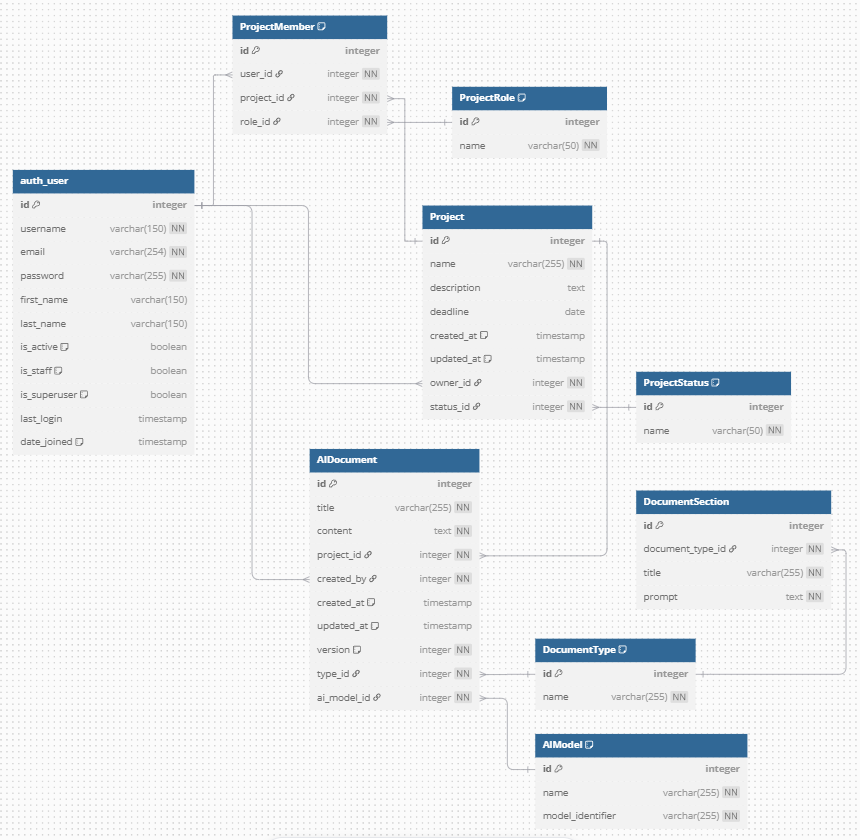
\includegraphics[width=\textwidth]{ERD.png}
            \label{fig-erd}
        \end{figure}
    \end{columns}
    % Az alkalmazás adatbázisának kialakítása során több táblát hoztam létre a különböző entitások tárolására.
    % - Felhasználók (auth_user): A felhasználók adatait tartalmazza, mint például a felhasználónevet, e-mail címet és jelszót.
    % - Projektek (Project): A létrehozott projektek adatait tárolja, beleértve a projekt nevét, leírását, határidejét, tulajdonosát és státuszát.
    % - Státuszok (ProjectStatus): A projektek aktuális állapotait tárolja, mint például „Draft”, „In Progress”, „Completed”.
    % - Szerepkörök (ProjectRole): A projektfeladatok során betöltött szerepköröket tartalmazza, mint például „Owner”, „Project Manager”, „Developer”, „Tester”, „Viewer”.
    % - Tagok (ProjectMember): A felhasználók kapcsolatait a projekthez tárolja, minden projekthez egy felhasználót egy szerepkörrel rendel.
    % - Dokumentum Típusok (DocumentType): A dokumentumok típusait és azokhoz tartozó sablonfájlok elérhetőségét tárolja, mint például „Specification” és „SRS”.
    % - Mesterséges Intelligencia Modellek (AIModel): A használt nyelvi modellek nevét és elérhetőségét tartalmazza, lehetővé téve azok egyszerű meghívását.
    % - Mesterséges Intelligencia Dokumentumok (AIDocument): A dokumentumok tartalmát és metaadatait, például címét, tartalmát és verzióját tárolja.
    % - Dokumentum Szekciók (DocumentSection): A dokumentumtípusokhoz tartozó szekciók adatait tartalmazza, beleértve a generálás során használt promptokat és a szekciók közötti függőségeket.
    
    % Az adatbázis kapcsolatai az alábbi típusok szerint lettek kialakítva:
    % - 1:N (egy-a-többhöz) kapcsolat: Például egy felhasználó több projektet is birtokolhat, de egy projektnek csak egy tulajdonosa lehet. Ehhez az auth_user és Project táblák közötti kapcsolatot használjuk, ahol az owner_id idegen kulcsként hivatkozik az auth_user táblában lévő elsődleges kulcsra (id).
    % - N:M (több-a-többhöz) kapcsolat: Például a felhasználók és projektek között több-a-többhöz kapcsolat van, amelyet a ProjectMember kapcsolótábla valósít meg.
    
    % Az adatbázis normalizálása a harmadik normálformára (3NF) történt, amely biztosítja a redundancia csökkentését és az adatkezelés hatékonyságát. Ennek során minden táblának van elsődleges kulcsa, és nincsenek tranzitív vagy részleges függőségek. Az adatbázis biztosítja az 1NF, 2NF és 3NF követelményeit, elkerülve a duplikált adatokat és biztosítva a hatékony lekérdezést.
    
    % Az adatbázis SQLite formátumban készült, mivel ez a rendszer gyors, önállóan működő, és kis méretének köszönhetően ideális kisebb webalkalmazásokhoz. Az SQLite platformfüggetlen és nem igényel külön SQL konfigurálást, mivel az adatbázis egyetlen fájlként tárolódik. Ezáltal egyszerűvé válik a migrációk kezelése és a biztonsági mentések készítése. Kisebb adatforgalmú alkalmazások számára ideális, mivel nincs szükség külső adatbázis-szerverre. Nagyobb forgalmú rendszerek esetén viszont nem ajánlott, mivel nem biztosítja a nagy számú párhuzamos lekérdezések hatékony kezelését.
\end{frame}

\begin{frame}{Osztályhierarchia}
    \vspace{-2em}
    \begin{columns}[t]
        \column{0.5\textwidth}
        \begin{itemize}
            \item Főbb osztályok:
                \begin{itemize}
                    \vspace{0.5em}
                    \item \textbf{views.py}
                    \vspace{0.5em}
                    \item \textbf{models.py}
                    \vspace{0.5em}
                    \item \textbf{forms.py}
                    \vspace{0.5em}
                    \item \textbf{urls.py}
                    \vspace{0.5em}
                    \item \textbf{settings.py}
                \end{itemize}
            \vspace{1em}
            \item Kapcsolatok:
                \begin{itemize}
                    \vspace{0.5em}
                    \item \texttt{views.py} $\leftrightarrow$ \texttt{models.py}
                    \vspace{0.5em}
                    \item \texttt{views.py} $\leftrightarrow$ \texttt{forms.py}
                    \vspace{0.5em}
                    \item \texttt{urls.py} $\rightarrow$ \texttt{views.py}
                \end{itemize}
        \end{itemize}
        % A \texttt{views.py} osztály kezeli a felhasználói kéréseket és válaszokat, az alkalmazás logikáját tartalmazza.
        % A \texttt{models.py} az adatbázis struktúráját és a kapcsolódó műveleteket tartalmazza.
        % A \texttt{forms.py} a felhasználói űrlapokat és azok validációját kezeli.
        % A \texttt{urls.py} az alkalmazás URL útvonalait és azokhoz rendelt nézeteket tartalmazza.
        % A \texttt{settings.py} az alkalmazás konfigurációját és beállításait kezeli.
        % A \texttt{views.py} osztály interakcióba lép a \texttt{models.py}-val, hogy adatokat kérjen le az adatbázisból.
        % A \texttt{views.py} osztály a \texttt{forms.py}-ban definiált űrlapokat használja a felhasználói adatbevitelhez.
        % A \texttt{urls.py} rendeli hozzá a kéréseket a megfelelő \texttt{views.py} funkciókhoz.
         \column{0.5\textwidth}
         \begin{figure}[ht!]
            \centering
            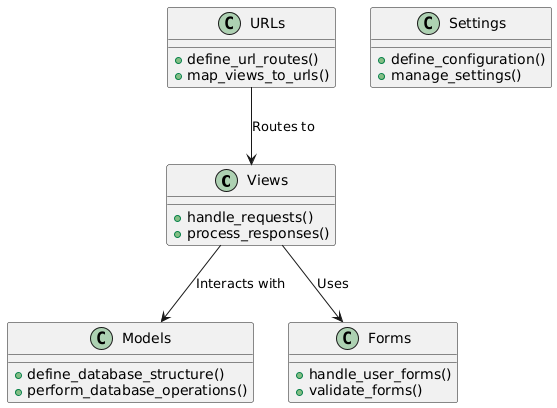
\includegraphics[width=\textwidth]{class_hierarchy.png}
            \label{fig-class-hierarchy}
        \end{figure}
        \vspace{-1.5em}
        \scriptsize
        Forrás: PlantUML alapú saját szerkesztés, a \url{https://plantuml.com/} oldalon, 2025
    \end{columns}
\end{frame}

\begin{frame}{A program fő funkciói/moduljai}
    \vspace{-2em}
    \begin{figure}[ht!]
        \centering
        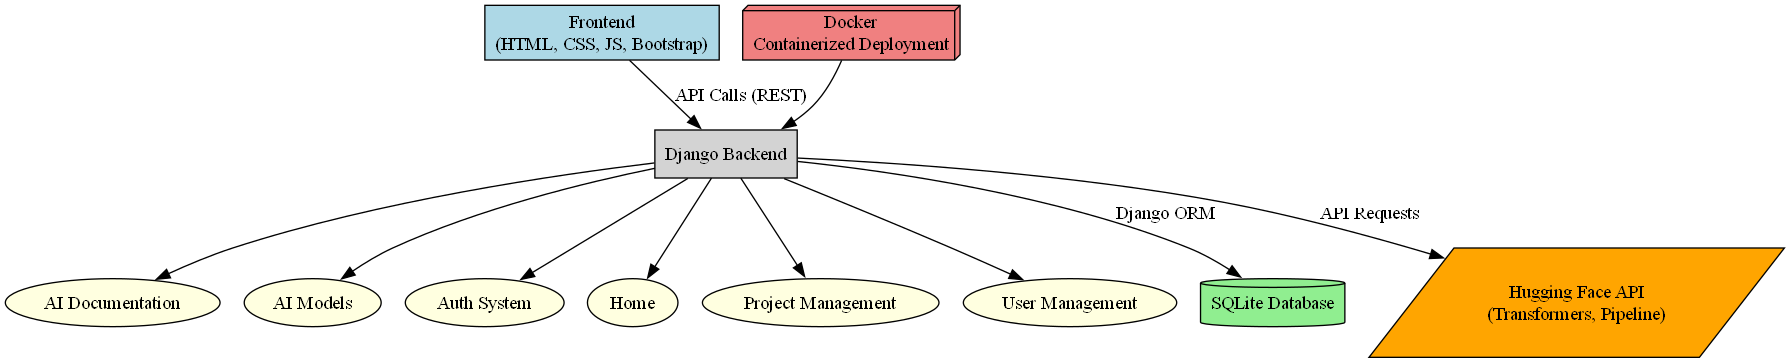
\includegraphics[width=\textwidth]{system_architecture.png}
           \label{fig-system-architecture}
    \end{figure}
    \vspace{-2em}
    \begin{center}
        \scriptsize
        Forrás: Graphviz dokumentáció alapján saját szerkesztés, 2025
    \end{center}
    \vspace{-1.5em}
    \begin{columns}[t]
        \column{0.5\textwidth}
        \begin{itemize}
            \item Fő funkciók
            \begin{itemize}
                \vspace{0.5em}
                \item Projektek kezelése
                \vspace{0.5em}
                \item Dokumentációk kezelése
                \vspace{0.5em}
                \item MI funkciók
                \vspace{0.5em}
                \item Profilkezelés
                \vspace{0.5em}
                \item Adminisztráció
            \end{itemize}
        \end{itemize}
        
        \column{0.5\textwidth}
        \begin{itemize}
            \item Felhasználói szerepkörök
            \begin{itemize}
                \vspace{0.5em}
                \item Vendég (Guest)
                \vspace{0.5em}
                \item Normál felhasználó (User)
                \vspace{0.5em}
                \item Moderátor (Staff)
                \vspace{0.5em}
                \item Adminisztrátor (Superuser)
            \end{itemize}
        \end{itemize}
    \end{columns}
    
    % Felhasználói szerepkörök:
    % - Vendég (Guest): Korlátozott hozzáférés, a regisztráció előtti tájékozódás céljából.
    % - Normál felhasználó (User): Teljes körű projekt- és dokumentációkezelés.
    % - Moderátor (Staff): Projektek és dokumentációk megtekintése, felhasználói támogatás.
    % - Adminisztrátor (Superuser): Teljes hozzáférés, felhasználók és rendszermodulok kezelése.
    
    % Fő funkciók:
    % - Projektek kezelése: Létrehozás, megtekintés, szerkesztés, törlés, tagok kezelése.
    % - Dokumentációk kezelése: Létrehozás, listázás, megtekintés, szerkesztés, törlés.
    % - MI funkciók: Cím- és leírásgenerálás, nyelvi modellek tesztelése.
    % - Profilkezelés: Regisztráció, bejelentkezés, adatmódosítás, kijelentkezés.
    % - Adminisztráció: Rendszeradminisztráció, felhasználók kezelése, adatbázis módosítása.
\end{frame}

\begin{frame}{Tesztelés}
    \begin{block}{Tesztelési módszerek}
        \begin{itemize}
            \vspace{0.5em}
            \item Egységtesztelés~(\textit{unit testing})
            \vspace{0.5em}
            \item Végponttól végpontig tartó tesztelés~(\textit{end-to-end testing}, \textsc{E2E})
            \vspace{0.5em}
        \end{itemize}
    \end{block}
    \begin{block}{\faChartBar~Tesztelési eredmények}
        \vspace{-1em}
        \begin{columns}[t]
            \column{0.45\textwidth}
            \begin{block}{\faFileCode~Egységtesztek}
              \begin{itemize}
                \vspace{0.5em}
                \item Tesztek száma: \textcolor{secondary}{248} db
                \vspace{0.5em}
                \item Időtartam: \textcolor{secondary}{4} perc \textcolor{secondary}{25,707} mp
                \vspace{0.5em}
                \item Eredmény: \textcolor{secondary}{Mind sikeres}
                \vspace{0.5em}
              \end{itemize}
            \end{block}
            \column{0.45\textwidth}
            \begin{block}{\faGlobe~E2E tesztek}
              \begin{itemize}
                \vspace{0.5em}
                \item Tesztek száma: \textcolor{secondary}{258} db
                \vspace{0.5em}
                \item Időtartam: \textcolor{secondary}{2} perc \textcolor{secondary}{27} mp
                \vspace{0.5em}
                \item Eredmény: \textcolor{secondary}{Mind sikeres}
                \vspace{0.5em}
              \end{itemize}
            \end{block}
        \end{columns}
    \end{block}

    % A tesztelési folyamat két fő formája az egységtesztelés (unit testing) és a végponttól végpontig tartó tesztelés (end-to-end testing, E2E) volt.
    % 
    % Egységtesztelés:
    % - A Django beépített unittest modulját használtam.
    % - Minden alkalmazáshoz külön tesztfájl készült, amely a modelleket, nézeteket, URL-eket, formokat és admin oldalt ellenőrzi.
    % - Az ai_models alkalmazás további teszteket tartalmaz a services.py fájlban található modellekre vonatkozóan.
    % - Példa teszt a PipelineTextGenerator osztály működésének ellenőrzésére: a tesztek vizsgálják, hogy a modell visszatér-e nem üres karakterlánccal és hogy a különböző hosszúságú generálások megfelelően működnek-e.
    %
    % Végponttól végpontig tartó tesztelés (E2E):
    % - A Cypress tesztkeretrendszert használtam.
    % - Minden oldalhoz külön almappákban találhatóak a tesztek, amelyek külön jogosultsági szintekre vannak bontva (guest, user, staff, superuser).
    % - Az E2E tesztek célja, hogy a teljes folyamatot a felhasználói szemszögből validálják.
    % - Minden jogosultsági szinthez tartozó funkció és megjelenített tartalom ellenőrizve van.
    % - Például a projektkezelő oldalak tesztelik a hozzáférési jogosultságokat és a helyes tartalmak megjelenítését.
\end{frame}

\subsection{Demo}
\begin{frame}{Demo - Rendszerbemutató}
\vspace{-1.5em}
  \begin{columns}[T]
    \begin{column}{0.45\textwidth}
      \begin{block}{\faUsers~ Projektek}
        \begin{itemize}
          \item Létrehozás, megtekintés, szerkesztés, törlés
          \item Tag- és jogosultságkezelés
        \end{itemize}
      \end{block}
      
      \begin{block}{\faUserShield~ Admin}
        \begin{itemize}
          \item Felhasználókezelés
          \item Rendszerbeállítások
        \end{itemize}
      \end{block}
    \end{column}
    
    \begin{column}{0.5\textwidth}
      \begin{block}{\faFileMedical~ Dokumentumok}
        \begin{itemize}
          \item Új dokumentumok létrehozása
          \item Szerkesztés, listázás, törlés, letöltés
        \end{itemize}
      \end{block}
      
      \begin{block}{\faUserCircle~ Profil}
        \begin{itemize}
          \item Regisztráció, bejelentkezés, kijelentkezés
          \item Adat- és jelszómódosítás
        \end{itemize}
      \end{block}
    \end{column}
  \end{columns}
\vspace{-0.5em}
  \begin{center}
      \begin{minipage}{0.5\textwidth}
        \begin{block}{\faRobot~ MI funkciók}
          \begin{itemize}
            \item Cím- és leírásgenerálás
            \item Nyelvi modellek tesztelése
          \end{itemize}
        \end{block}
      \end{minipage}
    \end{center}
\end{frame}

\begin{frame}{Főoldal áttekintés}
  \begin{center}
    \animategraphics[loop,autoplay,width=0.8\textwidth]{1}{gif/home/home_frame-}{0}{17}
  \end{center}
  \begin{itemize}
    \item \faHome~ Főmenü, gyorselérési csempék
    \item Áttekintés a legfontosabb funkciókról: projektek, dokumentumok, admin, MI
  \end{itemize}
  \begin{center}
    \scriptsize Forrás: Saját felvétel, 2025
  \end{center}
\end{frame}


\begin{frame}{Projektek kezelése}
    \begin{center}
      \animategraphics[loop,autoplay,width=0.8\textwidth]{0.5}{gif/projects/projects_frame-}{0}{19}
    \end{center}
    \begin{itemize}
      \item \faPlusCircle~Létrehozás, megtekintés, szerkesztés, törlés
      \item \faUsers~Tagok hozzáadása és jogosultságok kezelése
    \end{itemize}
    \begin{center}
        \scriptsize Forrás: Saját felvétel, 2025
    \end{center}
\end{frame}

\begin{frame}{Dokumentációk kezelése}
    \begin{center}
        \animategraphics[loop,autoplay,width=0.8\textwidth]{0.5}{gif/documents/documents_frame-}{0}{23}
    \end{center}
    \begin{itemize}
      \item \faFileMedical~Új dokumentumok létrehozása
      \item \faEdit~Szerkesztés, listázás, törlés, letöltés
    \end{itemize}
    \begin{center}
        \scriptsize Forrás: Saját felvétel, 2025
    \end{center}
\end{frame}

\begin{frame}{Profilkezelés}
    \begin{center}
        \animategraphics[loop,autoplay,width=0.8\textwidth]{0.5}{gif/profile_management/profile_management_frame-}{1}{32}
    \end{center}
    \begin{itemize}
      \item \faDoorOpen~Regisztráció, bejelentkezés, kijelentkezés
      \item \faUserEdit~Adatmódosítás és jelszócsere
    \end{itemize}
      \begin{center}
        \scriptsize Forrás: Saját felvétel, 2025
      \end{center}
\end{frame}

\begin{frame}{Adminisztráció}
    \begin{center}
      \animategraphics[loop,autoplay,width=0.8\textwidth]{0.5}{gif/admin/admin_frame-}{1}{8}
    \end{center}
    \begin{itemize}
      \item \faUserCog~Felhasználók kezelése
      \item \faCogs~Adatbázis módosítása, rendszeradminisztráció
    \end{itemize}
  \begin{center}
    \scriptsize Forrás: Saját felvétel, 2025
  \end{center}
\end{frame}

\begin{frame}{MI funkciók}
    \begin{center}
      \animategraphics[loop,autoplay,width=0.8\textwidth]{0.5}{gif/ai_function/ai_functions_frame-}{1}{51}
    \end{center}
    \begin{itemize}
      \item \faPen~Cím- és leírásgenerálás
      \item \faFlask~Nyelvi modellek tesztelése
    \end{itemize}
    \begin{center}
        \scriptsize Forrás: Saját felvétel, 2025
    \end{center}
\end{frame}

\section{Összegzés}

\begin{frame}{Elért eredmények a célkitűzésekkel összehasonlítva}
    \begin{columns}[T]
      \column{0.42\textwidth}
        \begin{block}{\faFlag~Célkitűzések}
          \small
          \begin{itemize}
            \vspace{0.5em}
            \item Ingyenes nyelvi modellek hatékony használata alacsony hardverigénnyel
            \vspace{0.5em}
            \item Minőségi dokumentációk és specifikációk generálása webalkalmazáson keresztül
            \vspace{0.5em}
            \item Intuitív, GitHub-kompatibilis dokumentumkezelés
            \vspace{0.5em}
          \end{itemize}
        \end{block}
      \column{0.06\textwidth}
        \vspace{8em}
        \centering
        
\includegraphics[width=0.8\textwidth]{arrow-right-arrow-left-solid.png}
      \column{0.42\textwidth}
        \begin{block}{\faCheckCircle~Elért eredmények}
          \small
          \begin{itemize}
            \vspace{0.5em}
            \item Jelentős minőségjavulás specifikus promptolási technikákkal
            \vspace{0.5em}
            \item Gyors és egyszerű Markdown dokumentumgenerálás GitHub kompatibilitással
            \vspace{0.5em}
            \item Komplex összefüggések kezelése korlátozott, további finomhangolás szükséges
            \vspace{0.5em}
          \end{itemize}
        \end{block}
    \end{columns}
    % A célom egy olyan webalkalmazás fejlesztése volt, amely ingyenes nyelvi modellekkel, alacsony hardverigény mellett képes minőségi dokumentációkat és specifikációkat generálni, egyszerűen kezelhető felületen.
    % Specifikus promptolási technikák és paraméterbeállítások alkalmazásával jelentős javulást értem el a generált szövegek minőségében, de a kisebb modellek teljesítménye elmarad a nagyobb modellekétől.
    % A rendszer gyors és intuitív Markdown alapú dokumentumgenerálást biztosít, amely kompatibilis a GitHub platformmal, így hatékonyan támogatja a projektmenedzsmentet.
    % A generált szövegek azonban még nem képesek komplexebb összefüggések kezelésére, ezért a jövőbeni fejlesztések fókuszában a modellek finomhangolása és a komplexitás növelése áll.
\end{frame}

\begin{frame}{További fejlesztési lehetőségek}
    \vspace{-1em}
    \begin{itemize}
        \vspace{1.5em}
        \item[\faCogs] Specifikus finomhangolás dokumentumtípusokra
        \vspace{1.5em}
        \item[\faSlidersH] Feladatspecifikus prompt- és paraméteroptimalizálás
        \vspace{1.5em}
        \item[\faFile] További dokumentumtípusok integrálása
        \vspace{1.5em}
        \item[\faCheckCircle] Automatikus tartalomértékelés és iteratív finomhangolás
        \vspace{1.5em}
        \item[\faDatabase] Vektoradatbázis-alapú kontextuskezelés (\textsc{RAG})
        \vspace{1.5em}
        \item[\faTools] Rendszer- és futási teljesítmény optimalizálása
    \end{itemize}
    % Specifikus finomhangolás dokumentumtípusokra: A modellek teljesítménye javítható célzott, dokumentumtípus-specifikus adatokkal történő finomhangolással, bár az ilyen adatok gyakran nem nyilvánosak vagy eltérő formátumban érhetők el, ami kihívást jelent.
    % Feladatspecifikus prompt- és paraméteroptimalizálás: A generált szövegek minőségét és relevanciáját a promptok és paraméterek feladathoz igazított finomhangolásával lehetne növelni.
    % További dokumentumtípusok integrálása: A rendszer bővíthető új dokumentumtípusokkal, például \texttt{Vision Statement}, \texttt{Design Document}, \texttt{Test Plan} vagy \texttt{User Manual}, amelyek eltérő szerkezeti és nyelvi logikát igényelnek, növelve az alkalmazhatóságot.
    % Automatikus tartalomértékelés és iteratív finomhangolás: Egy közepes méretű modell alkalmazásával a generált tartalom automatikusan értékelhető, majd iteratívan finomhangolható, ami erőforrás-igényes, de jelentős minőségjavulást hozhat.
    % Vektoradatbázis-alapú kontextuskezelés (\textsc{RAG}): A vektoradatbázis integrációja lehetővé tenné a hasonló szövegek kontextusba vonását, javítva a generálás pontosságát és relevanciáját.
    % Rendszer- és futási teljesítmény optimalizálása: A generálási folyamatok gyorsíthatók lokális \textsc{GPU} vagy felhőalapú megoldásokkal, illetve a sablonok és adatbázisok tartalmi bővítésével.
\end{frame}

\section{Opponens kérdései}
\begin{frame}{Opponens kérdései}
    \textcolor{gray}{\textbf{Dr. Tajti Tibor Gábor}}
    \vspace{1em}
    \begin{block}{Kérdés szöveg…}
        \small
        Válasz szöveg…
    \end{block}
    \vspace{1em}
    \begin{block}{Kérdés szöveg…}
        \small
        Válasz szöveg…
    \end{block}
\end{frame}


\section*{}
\begin{frame}
    \setbeamertemplate{footline}{}
    \begin{tikzpicture}[remember picture,overlay]
        \node[anchor=center, inner sep=0pt] at (current page.center)
          {
\includegraphics[width=\paperwidth, height=\paperheight, keepaspectratio]{ekke_logo.png}};
        \fill[fill=background, fill opacity=0.9] (current page.south west) rectangle (current page.north east);
    \end{tikzpicture}
    \vfill
    \begin{center}
        
\includegraphics[width=0.2\textwidth]{robot-solid.png}\\
        \vspace{1em}
        \Huge\bfseries\color{primary}Köszönöm a figyelmet!\\[1cm]
        \normalsize\insertauthor
    \end{center}
    \vfill
\end{frame}

\end{document}